\documentclass{article}



\usepackage{arxiv}

\usepackage[utf8]{inputenc} % allow utf-8 input
\usepackage[T1]{fontenc}    % use 8-bit T1 fonts
\usepackage{hyperref}       % hyperlinks
\usepackage{url}            % simple URL typesetting
\usepackage{booktabs}       % professional-quality tables
\usepackage{amsfonts}       % blackboard math symbols
\usepackage{nicefrac}       % compact symbols for 1/2, etc.
\usepackage{microtype}      % microtypography
\usepackage{lipsum}		% Can be removed after putting your text content
\usepackage{graphicx}
\usepackage[super]{natbib}
\usepackage{doi}
\usepackage{float}
\usepackage{amsmath}
\usepackage{mathrsfs}
\usepackage{caption} 
\usepackage{multicol}
\usepackage{pgfplots}
\usepackage{sectsty}
\usepackage{cancel}
\usepackage{amsmath}
\usepackage{amssymb}
\usepackage{listings}
\usepackage{algorithm}
\usepackage{algpseudocode}
\DeclareUnicodeCharacter{2212}{-}
\usetikzlibrary{patterns}
\usetikzlibrary{calc}


\title{\emph{Randomized Algorithm}}

\newcommand{\mycomment}[1]{}
\NewDocumentCommand{\codeword}{v}{%
\texttt{\textcolor{blue}{#1}}%
}


%\date{September 9, 1985}	% Here you can change the date presented in the paper title
%\date{} 					% Or removing it

\author{{\hspace{1mm}Rajat Dua} \\
	Master of Science - Computer Science\\
	Aarhus University\\
	\texttt{au747653@uni.au.dk / 202303549@post.au.dk} \\
	%% examples of more authors
	\And
	{\hspace{1mm}Kasper Green Larsen} \\
	Institut for Datalogi\\
	Aarhus University\\
	%% \AND
	%% Coauthor \\
	%% Affiliation \\
	%% Address \\
	%% \texttt{email} \\
	%% \And
	%% Coauthor \\
	%% Affiliation \\
	%% Address \\
	%% \texttt{email} \\
	%% \And
	%% Coauthor \\
	%% Affiliation \\
	%% Address \\
	%% \texttt{email} \\
}

% Uncomment to remove the date
\date{February 5, 2024}

% Uncomment to override  the `A preprint' in the header
\renewcommand{\headeright}{Rajat Dua}
\renewcommand{\undertitle}{Week 7 - Hash Functions}
\renewcommand{\shorttitle}{\textit{Randomized Algorithm} Notes}

%%% Add PDF metadata to help others organize their library
%%% Once the PDF is generated, you can check the metadata with
%%% $ pdfinfo template.pdf
\hypersetup{
pdftitle={Randomized Algorithm},
pdfsubject={q-bio.NC, q-bio.QM},
pdfauthor={Rajat Dua},
pdfkeywords={randomized, notes, au, aarhus, university},
}
\captionsetup[table]{skip=10pt}

% \subsectionfont{\underline}


\begin{document}
\maketitle
\vspace{-1cm}
\section{Overview}

\subsection{Hash Function Definition}

$$
h:[U] \rightarrow [m]
$$

Where $h$ is a truly random hashing function which isn't practical. 

\subsection{Properties}

$h$ is universal if

$$
\forall_{x\neq y} \in [U]: Pr_{h} [h(x) = h(y)] \leq \frac{1}{m}
$$

$c$-approximate universal if:

$$
\forall_{x\neq y}[U]: Pr_{h}[h(x) = h(y)] \leq \frac{c}{m}
$$

For any constant $c$, it can be $2, \ldots \mathbb N$

\subsection{Recap}

In a set $S$ there are keys $(x_1, \ldots, x_n)$ and we did the expectation of $x \in S$ to find the collision:

$$
X = |List(A[h(x)])|
$$

Where the RV was

$$
X_i = \left\{
\begin{matrix}
    1, && h(x) = h(x_i) \\
    0, && \text{otherwise}
\end{matrix}
\right\}
$$

And the expectation was:

$$
\mathbb E_h[X] = \mathbb E_h [\sum^{n}_{i=1} X_i] = \sum_{i=1}^{n} \mathbb E[X_i] = \sum_{i=1}^{n} Pr_{h}[h(x) = h(x_i)]
$$

Using linearity of expectation.

\subsection{C-approximate Hash Function}

We can then plug the universal definition to get upper bound by $\frac{c}{m}$

$$
\sum_{i=1}^{n} Pr_{h}[h(x) = h(x_i)] \leq 1 + \sum^{n}_{{i=1}_{x \neq x_i}} \frac{c}{m} = 1 + c \frac{n}{m} = 1 + c
$$

For $n = m$. For $c = 3$, the hash function is $3$-approximate universal.

\section{Signatures as Hash Values}
For keys $x_1, \ldots, x_n \in U$ we can define signatures as $S(x_1), \ldots, S(x_n)$ such that you can try to compare $S(x_i) \neq S(x_j)$ between two parties. Instead of sending the whole file, you can just compare the signature and see if you have the file or not.

In short, we want to assign a signature to a key. The reason to do it is because if we want to assign a large string to a smaller value which is what signature can help.

\subsection{How to define these signatures?}

Hash function ($S$): $U \rightarrow [n^3]$ and let's say $S: c$-approximate universal. We can say this gives a "good" signature with good probability.

$$
Pr_{S}[\exists_{i\neq j}: S(x_i) = S(x_j)]
$$

Here we can use Union bound since we are working with events that we want to avoid that collision. So, above expression can be represented using $E_{ij} = \{S(x_i) = S(x_j)\}$ as follows:

$$
= Pr_{S}[\cup_{i \neq j} E_{ij}] \leq \sum_{i \neq j} Pr[E_{ij}]
$$

Since we are working with an output range of $n^3$ and $c$-approximate universal. So, what is the probability of $E_{i} = E_{ij}$ basically the we want to define $Pr_{S}[\exists_{i\neq j}: S(x_i) = S(x_j)]$ so it is $c$-approximate universal so its $\frac{c}{n}$ and we are working with $n^3$ so it will be $\frac{c}{n^3}$. Represented as follows:

$$
\leq \sum_{i = j} \frac{c}{n^3} \leq \frac{n^2}{2} \cdot \frac{c}{n^3} \leq \frac{c}{2} \cdot \frac{1}{n}
$$

\textbf{How is the sum $\frac{n^2}{2}$?}

The number of such pairs is given by the combination formula $\left(\begin{matrix}
    n \\
    2
\end{matrix}\right)$, which is $\frac{n(n-1)}{2}$ that is approximately $\frac{n^2}{2}$ for large $n$

There is a very small chance.

$$
= \frac{c}{2T}
$$

I have a very large $T$ the chance will be really small.

Universe of strings with very long length and we are working with $c$-approx universal $S$. For $T = 2^64$, then the probability:

$$
Pr_{S}[\exists_{i\neq j}: S(x_i) = S(x_j)] \leq 2^{-64}
$$

So, it is never going to happen.

So, if we have $n = 10^6$ records we want to store, which is approximately $2^{20}$ which for the output space $n^2 \cdot T$ will be $2^{20} \cdot 2^{20} \cdot 2^{64} = 2^{104}$ which is saying that you can store the full-text file document as a signature that is $104$ bits and it's not very long, so you can save space instead of storing the file as it is. 

We just have to agree with a hash function. Another motivation for hashing \^.

\section{Hashing Integers}

$h:[U] \rightarrow [m]$, pick $p > U$ and you also pick $a \in_{R} {[p]}_{+} = \{1, \ldots, p-1\}$ and $b \in_{R} {[p]} = \{0, \ldots, p-1\}$. Where $\in_{R}$ is uniformly random. We will know later why $a$ is not in ${[p]}$ or why $a$ can't be $0$.

We define the hash function with $a,b$ as follows:

$$
h_{(a,b)}(x) = (a \cdot x + b \mod p) \mod m
$$

We $\mod m$ to get a number between $0$ and $m-1$.

So, why is this a universal hash function? We will make the same argument that collision is minimal. This can be written as:

$$
\forall_{x\neq y} \in [U]: Pr_{a,b} [h_{a,b}(x) = h_{a,b}(y)] < \frac{1}{m}
$$

\textbf{Note}: that it is $<$ and not $\leq$ so it is even better than a truly random hash function which had $ \leq 
 \frac{1}{m}$

 \subsection{Understanding first part - $a \cdot x + b \mod p$}

For a pair $x \neq y$ and $(a,b)$, let's write equations as follows:

\begin{align*}
    a \cdot x + b \equiv q \mod p \\
    a \cdot y + b \equiv r \mod p
\end{align*}

We want to see what happens to $x$ if we do $a \cdot x + b \mod p$ and what happens to $y$ if we do $a \cdot y + b \mod p$. With the equation above we get $q$ and $r$ respectively and we are trying to find out the relation between $(a,b)$ pair for $(q,r)$. To do that, we need to know the number theory fact.

\textbf{$\mathbf{FACT}$: If $p$ is prime and $\alpha, \beta \in {[p]}_{+}$ then $\alpha \cdot \beta \not\equiv 0 \mod p$}


We make a \textbf{claim} that, if there is a fixed $(x,y)$ there is 1-1 correspondence between pairs $(a,b) \in [p] \times [p]$ and put $(q,r) \in [p] \times [p]$

To prove the above statement. Let's pick a pair $(q,r)$ and show that there is only one pair $(a,b)$ which is valid for the above equations.

\textbf{For pair $(a,b)$}:

\begin{equation}\label{week7-pair-ab-q}
    a \cdot x + b \equiv q \mod p
\end{equation}
\begin{equation}\label{week7-pair-ab-r}
    a \cdot y + b \equiv r \mod p
\end{equation}

If we subtract \eqref{week7-pair-ab-q} and  \eqref{week7-pair-ab-r} we get:

\begin{equation}\label{week7-pair-ab-qr-sub}
    a \cdot (x-y) \equiv q - r \mod p
\end{equation}

\textbf{For pair $(a',b')$}:

\begin{equation}\label{week7-pair-ab-prime-q}
    a' \cdot x + b' \equiv q \mod p
\end{equation}
\begin{equation}\label{week7-pair-ab-prime-r}
    a' \cdot y + b' \equiv r \mod p
\end{equation}

If we subtract \eqref{week7-pair-ab-prime-q} and  \eqref{week7-pair-ab-prime-r} we get:

\begin{equation}\label{week7-pair-ab-prime-qr-sub}
    a' \cdot (x-y) \equiv q - r \mod p
\end{equation}

If we subtract \eqref{week7-pair-ab-qr-sub} and \eqref{week7-pair-ab-prime-qr-sub}, we get:

$$
(a-a')(x-y) \equiv 0 \mod p
$$

For this equation, we know $x-y \neq 0$ because $x\neq y$ is mentioned in the beginning. So, $a = a' \equiv 0 \mod p$ which means that $a = a'$

Now, to argue for $b$ and $b'$, let's subtract \eqref{week7-pair-ab-q} and \eqref{week7-pair-ab-prime-q} from which we get:

$$
b-b' \equiv 0 \mod p
$$

For this equation, we can simply say $b = b'$. Therefore we can say two things from this proof so far:

\begin{enumerate}
    \item For any $(q,r)$ there is \textbf{at most one} pair $(a,b)$
    \item For every $(a,b)$ it gives same $(q,r)$
    \item For every $(a,b)$ that is picked uniformly random in $[p] \times [p]$ means that $(q,r)$ is picked uniformly random in $[p] \times [p]$
\end{enumerate}

If $a = 0$, then the hash value doesn't depend on the key that's why $a \in_{R} {[p]}_{+}$.

For $(a,b) \in_{R} {[p]}_{+} \times [p]$, we make a claim that if $a \neq 0$ then $q \neq r$. How can we show that? Let's take the \eqref{week7-pair-ab-prime-qr-sub} and compare the same equation with a scenario when $q = r$ will result in:

$$
a \cdot (x-y) \equiv 0 \mod p
$$

Which states that $x-y \neq 0$ because $x \neq y$. So, $a = 0$. Therefore, there is an independence between $a \neq 0$ so $q \neq r$.

So, we get to know that this FIRST PART is uniformly random. $(a\cdot x + b \mod p, a \cdot y + b \mod p)$ is uniformly random among $(q,r) \in_{R} {[p]}_{+} \times [p]$ with $q \neq r$

\subsection{Understanding second part - $\mod m$ of first part}

If we take a fixed $q$, then how many values of $r$ collide with $q \mod m$ basically stating:

$$
r \equiv q \mod m
$$

That will help us find the question we want to answer about collision $h_{a,b}(x) = h_{a,b}(y)$. We can visualise what are the possible "buckets" that $q$ can fall under when we are doing $\mod m$. 

\begin{figure}[h]
    \centering
    

\tikzset{every picture/.style={line width=0.75pt}} %set default line width to 0.75pt        

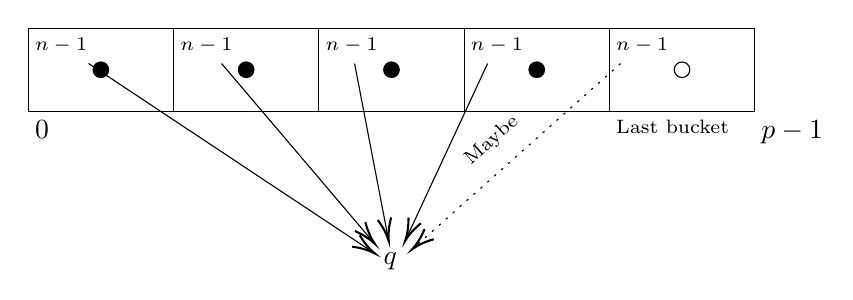
\begin{tikzpicture}[x=0.75pt,y=0.75pt,yscale=-1,xscale=1]
%uncomment if require: \path (0,300); %set diagram left start at 0, and has height of 300

%Shape: Rectangle [id:dp2677152332750321] 
\draw   (437,129) -- (507,129) -- (507,169) -- (437,169) -- cycle ;
%Shape: Rectangle [id:dp7833886011805218] 
\draw   (157,129) -- (227,129) -- (227,169) -- (157,169) -- cycle ;
%Shape: Rectangle [id:dp7310415488806259] 
\draw   (297,129) -- (367,129) -- (367,169) -- (297,169) -- cycle ;
%Shape: Rectangle [id:dp7366652753440439] 
\draw   (227,129) -- (297,129) -- (297,169) -- (227,169) -- cycle ;
%Shape: Rectangle [id:dp6367104530688215] 
\draw   (367,129) -- (437,129) -- (437,169) -- (367,169) -- cycle ;
%Shape: Circle [id:dp7964161760285873] 
\draw  [fill={rgb, 255:red, 0; green, 0; blue, 0 }  ,fill opacity=1 ] (188.25,149) .. controls (188.25,146.93) and (189.93,145.25) .. (192,145.25) .. controls (194.07,145.25) and (195.75,146.93) .. (195.75,149) .. controls (195.75,151.07) and (194.07,152.75) .. (192,152.75) .. controls (189.93,152.75) and (188.25,151.07) .. (188.25,149) -- cycle ;
%Shape: Circle [id:dp8246219367906953] 
\draw  [fill={rgb, 255:red, 0; green, 0; blue, 0 }  ,fill opacity=1 ] (258.25,149) .. controls (258.25,146.93) and (259.93,145.25) .. (262,145.25) .. controls (264.07,145.25) and (265.75,146.93) .. (265.75,149) .. controls (265.75,151.07) and (264.07,152.75) .. (262,152.75) .. controls (259.93,152.75) and (258.25,151.07) .. (258.25,149) -- cycle ;
%Shape: Circle [id:dp6268923279844762] 
\draw  [fill={rgb, 255:red, 0; green, 0; blue, 0 }  ,fill opacity=1 ] (328.25,149) .. controls (328.25,146.93) and (329.93,145.25) .. (332,145.25) .. controls (334.07,145.25) and (335.75,146.93) .. (335.75,149) .. controls (335.75,151.07) and (334.07,152.75) .. (332,152.75) .. controls (329.93,152.75) and (328.25,151.07) .. (328.25,149) -- cycle ;
%Shape: Circle [id:dp7410319870316375] 
\draw  [fill={rgb, 255:red, 0; green, 0; blue, 0 }  ,fill opacity=1 ] (398.25,149) .. controls (398.25,146.93) and (399.93,145.25) .. (402,145.25) .. controls (404.07,145.25) and (405.75,146.93) .. (405.75,149) .. controls (405.75,151.07) and (404.07,152.75) .. (402,152.75) .. controls (399.93,152.75) and (398.25,151.07) .. (398.25,149) -- cycle ;
%Shape: Circle [id:dp12782242697658286] 
\draw  [fill={rgb, 255:red, 255; green, 255; blue, 255 }  ,fill opacity=1 ] (468.25,149) .. controls (468.25,146.93) and (469.93,145.25) .. (472,145.25) .. controls (474.07,145.25) and (475.75,146.93) .. (475.75,149) .. controls (475.75,151.07) and (474.07,152.75) .. (472,152.75) .. controls (469.93,152.75) and (468.25,151.07) .. (468.25,149) -- cycle ;

% Text Node
\draw (159,172.4) node [anchor=north west][inner sep=0.75pt]    {$0$};
% Text Node
\draw (509,172.4) node [anchor=north west][inner sep=0.75pt]    {$p-1$};
% Text Node
\draw (229,132.4) node [anchor=north west][inner sep=0.75pt]  [font=\scriptsize]  {$n-1$};
% Text Node
\draw (299,132.4) node [anchor=north west][inner sep=0.75pt]  [font=\scriptsize]  {$n-1$};
% Text Node
\draw (369,132.4) node [anchor=north west][inner sep=0.75pt]  [font=\scriptsize]  {$n-1$};
% Text Node
\draw (439,132.4) node [anchor=north west][inner sep=0.75pt]  [font=\scriptsize]  {$n-1$};
% Text Node
\draw (327,235.9) node [anchor=north west][inner sep=0.75pt]    {$q$};
% Text Node
\draw (159,132.4) node [anchor=north west][inner sep=0.75pt]  [font=\scriptsize]  {$n-1$};
% Text Node
\draw (364.22,190.2) node [anchor=north west][inner sep=0.75pt]  [rotate=-318.28] [align=left] {{\scriptsize Maybe}};
% Text Node
\draw (439,172) node [anchor=north west][inner sep=0.75pt]  [font=\scriptsize] [align=left] {Last bucket};
% Connection
\draw    (186.06,146) -- (322.33,236.42) ;
\draw [shift={(324,237.53)}, rotate = 213.57] [color={rgb, 255:red, 0; green, 0; blue, 0 }  ][line width=0.75]    (10.93,-3.29) .. controls (6.95,-1.4) and (3.31,-0.3) .. (0,0) .. controls (3.31,0.3) and (6.95,1.4) .. (10.93,3.29)   ;
% Connection
\draw    (250.15,146) -- (322.7,231.38) ;
\draw [shift={(324,232.91)}, rotate = 229.64] [color={rgb, 255:red, 0; green, 0; blue, 0 }  ][line width=0.75]    (10.93,-3.29) .. controls (6.95,-1.4) and (3.31,-0.3) .. (0,0) .. controls (3.31,0.3) and (6.95,1.4) .. (10.93,3.29)   ;
% Connection
\draw    (314.23,146) -- (330.31,229.54) ;
\draw [shift={(330.69,231.5)}, rotate = 259.1] [color={rgb, 255:red, 0; green, 0; blue, 0 }  ][line width=0.75]    (10.93,-3.29) .. controls (6.95,-1.4) and (3.31,-0.3) .. (0,0) .. controls (3.31,0.3) and (6.95,1.4) .. (10.93,3.29)   ;
% Connection
\draw    (378.32,146) -- (339.42,229.69) ;
\draw [shift={(338.58,231.5)}, rotate = 294.93] [color={rgb, 255:red, 0; green, 0; blue, 0 }  ][line width=0.75]    (10.93,-3.29) .. controls (6.95,-1.4) and (3.31,-0.3) .. (0,0) .. controls (3.31,0.3) and (6.95,1.4) .. (10.93,3.29)   ;
% Connection
\draw  [dash pattern={on 0.84pt off 2.51pt}]  (442.4,146) -- (343.49,234.15) ;
\draw [shift={(342,235.48)}, rotate = 318.29] [color={rgb, 255:red, 0; green, 0; blue, 0 }  ][line width=0.75]    (10.93,-3.29) .. controls (6.95,-1.4) and (3.31,-0.3) .. (0,0) .. controls (3.31,0.3) and (6.95,1.4) .. (10.93,3.29)   ;

\end{tikzpicture}

\end{figure}


When we make buckets from $0 \rightarrow p-1$ for $i$ offsets, it is not necessary that the $q$ would fall in the last bucket. So, if there are $p$ possible choices and out of $m$ space for $r \in [p]$:

$$
\lceil\frac{p}{m}\rceil
$$
and since the last bucket is not always possible, the probability is minimal. So, we can say the number of $r \in [p]\{q\}$ (excluding singular $q$) for $r \mod m = q \mod m$:

$$
\lceil\frac{p}{m}\rceil - 1
$$

Using number theory we know that, if we try to round up:

$$
\lceil\frac{v}{m}\rceil \leq \frac{v+m-1}{m}
$$

So, we can say:

$$
\lceil\frac{p}{m}\rceil - 1 \leq \frac{p+m-1}{m} = \frac{p-1}{m}
$$

Therefore, the number of pairs $(q,r)$ with $r\neq q$ that collide with $\mod m$ is $\leq \frac{p(p-1)}{m}$. We know that we are working with ${[p]}_{+} \times [p]$ so there are possible $p(p-1)$ pairs. So, we can say that the probability of collision is:

$$
Pr[\text{ That there is a collision }] = \frac{\frac{p(p-1)}{m}}{p(p-1)} \leq \frac{1}{m}
$$

But why $\leq$ we mentioned it should have been $<$ since the probability to fall under the last bucket is minimal which is why did minus $1$. There has to be one pair where a number of collisions is at most rounded down:

$$
\lfloor\frac{p}{m}\rfloor - 1 < \lceil\frac{p}{m}\rceil - 1
$$

\subsection{Practical implementation}

This is very frustrating to implement. Let's say we want to hash a $64$ bit integer ($2^{64}$). We want $p > u$ so it doesn't collide, $p$ is prime. So, $p > 2^{64}$.

The size of $a,b$ can be $> 2^{64}$ so this means that $a \cdot x$ will result in $128$ bits which wouldn't fit in a $64$ bit integer.

To fix this, one can use chunking of $a$ and $x$ in chunks of $32$-bits. After chunking, then you can use the old-school multiplying which isn't efficient since you have to work with carries and bit shifts with $0$s to do the old-school addition that you get with multiplication. However, that was only one part of the whole expression. We also need to do $\mod p$ after we are done with the multiplication.

\begin{figure}[h]
    \centering
    

\tikzset{every picture/.style={line width=0.75pt}} %set default line width to 0.75pt        

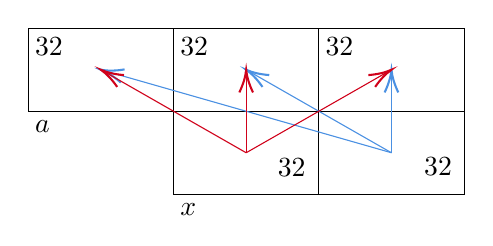
\begin{tikzpicture}[x=0.75pt,y=0.75pt,yscale=-1,xscale=1]
%uncomment if require: \path (0,300); %set diagram left start at 0, and has height of 300

%Shape: Rectangle [id:dp5276050870394144] 
\draw   (230,94) -- (300,94) -- (300,134) -- (230,134) -- cycle ;
%Shape: Rectangle [id:dp6070662025699092] 
\draw   (300,94) -- (370,94) -- (370,134) -- (300,134) -- cycle ;
%Shape: Rectangle [id:dp5331198652287072] 
\draw   (370,94) -- (440,94) -- (440,134) -- (370,134) -- cycle ;
%Shape: Rectangle [id:dp035559195025739676] 
\draw   (300,134) -- (370,134) -- (370,174) -- (300,174) -- cycle ;
%Shape: Rectangle [id:dp48345974395710156] 
\draw   (370,134) -- (440,134) -- (440,174) -- (370,174) -- cycle ;
%Straight Lines [id:da22007269489451353] 
\draw [color={rgb, 255:red, 74; green, 144; blue, 226 }  ,draw opacity=1 ]   (405,154) -- (405,116) ;
\draw [shift={(405,114)}, rotate = 90] [color={rgb, 255:red, 74; green, 144; blue, 226 }  ,draw opacity=1 ][line width=0.75]    (10.93,-3.29) .. controls (6.95,-1.4) and (3.31,-0.3) .. (0,0) .. controls (3.31,0.3) and (6.95,1.4) .. (10.93,3.29)   ;
%Straight Lines [id:da8664775122742399] 
\draw [color={rgb, 255:red, 74; green, 144; blue, 226 }  ,draw opacity=1 ]   (405,154) -- (336.74,114.99) ;
\draw [shift={(335,114)}, rotate = 29.74] [color={rgb, 255:red, 74; green, 144; blue, 226 }  ,draw opacity=1 ][line width=0.75]    (10.93,-3.29) .. controls (6.95,-1.4) and (3.31,-0.3) .. (0,0) .. controls (3.31,0.3) and (6.95,1.4) .. (10.93,3.29)   ;
%Straight Lines [id:da0526687282790812] 
\draw [color={rgb, 255:red, 74; green, 144; blue, 226 }  ,draw opacity=1 ]   (405,154) -- (266.92,114.55) ;
\draw [shift={(265,114)}, rotate = 15.95] [color={rgb, 255:red, 74; green, 144; blue, 226 }  ,draw opacity=1 ][line width=0.75]    (10.93,-3.29) .. controls (6.95,-1.4) and (3.31,-0.3) .. (0,0) .. controls (3.31,0.3) and (6.95,1.4) .. (10.93,3.29)   ;
%Straight Lines [id:da9456754862436691] 
\draw [color={rgb, 255:red, 208; green, 2; blue, 27 }  ,draw opacity=1 ]   (335,154) -- (403.26,114.99) ;
\draw [shift={(405,114)}, rotate = 150.26] [color={rgb, 255:red, 208; green, 2; blue, 27 }  ,draw opacity=1 ][line width=0.75]    (10.93,-3.29) .. controls (6.95,-1.4) and (3.31,-0.3) .. (0,0) .. controls (3.31,0.3) and (6.95,1.4) .. (10.93,3.29)   ;
%Straight Lines [id:da11807798058126884] 
\draw [color={rgb, 255:red, 208; green, 2; blue, 27 }  ,draw opacity=1 ]   (335,154) -- (335,116) ;
\draw [shift={(335,114)}, rotate = 90] [color={rgb, 255:red, 208; green, 2; blue, 27 }  ,draw opacity=1 ][line width=0.75]    (10.93,-3.29) .. controls (6.95,-1.4) and (3.31,-0.3) .. (0,0) .. controls (3.31,0.3) and (6.95,1.4) .. (10.93,3.29)   ;
%Straight Lines [id:da02021759078099472] 
\draw [color={rgb, 255:red, 208; green, 2; blue, 27 }  ,draw opacity=1 ]   (335,154) -- (266.74,114.99) ;
\draw [shift={(265,114)}, rotate = 29.74] [color={rgb, 255:red, 208; green, 2; blue, 27 }  ,draw opacity=1 ][line width=0.75]    (10.93,-3.29) .. controls (6.95,-1.4) and (3.31,-0.3) .. (0,0) .. controls (3.31,0.3) and (6.95,1.4) .. (10.93,3.29)   ;

% Text Node
\draw (232,137.4) node [anchor=north west][inner sep=0.75pt]    {$a$};
% Text Node
\draw (302,177.4) node [anchor=north west][inner sep=0.75pt]    {$x$};
% Text Node
\draw (232,97.4) node [anchor=north west][inner sep=0.75pt]    {$32$};
% Text Node
\draw (302,97.4) node [anchor=north west][inner sep=0.75pt]    {$32$};
% Text Node
\draw (372,97.4) node [anchor=north west][inner sep=0.75pt]    {$32$};
% Text Node
\draw (349,155.4) node [anchor=north west][inner sep=0.75pt]    {$32$};
% Text Node
\draw (419.5,154.9) node [anchor=north west][inner sep=0.75pt]    {$32$};


\end{tikzpicture}

    \caption{Old School Multiplication}
\end{figure}

However, there is a way to make it efficient on the basis of how you pick $p$. If you mick \textbf{Mersenne Prime} we can $\mod$ it easily. Some examples of these kinds of prime - $2^{61} - 1, 2^{89} - 1$. 

Let's see why it is a useful prime, it gives. Let's say we want to calculate a mersenne prime number such that we have $p = 2^{q} - 1$

Then we can say we write ($2^q = p + 1$):

\begin{align*}
    x \mod p = 2^q - 1 \\
    x = x \mod 2^q + 2^q \lfloor\frac{x}{2^q}\rfloor \\
    x = x \mod 2^q + (p+1) \lfloor\frac{x}{2^q}\rfloor \\
    x \mod p = (x \mod 2^q + \lfloor\frac{x}{2^q}\rfloor) \mod p \\
\end{align*}

\textbf{Reason}: $p+1$ isn't there because we are working with $\mod p$

$x \mod 2^q$: represents the $q$ least significant bits. (Binary number which is modulo by $2$) \\
$\lfloor\frac{x}{2^q}\rfloor$: round down in terms of binary represents the most significant bits but shifted towards an LSB position.

In C, you can do this expression very quickly. It uses \codeword{Unsigned Int} with this:

$$
x \: \& \: p + x >>p
$$

$x$ bitwise AND $p$, where $p$ is $1111100000$ so if we do bitwise AND we get $XXXXXX000000$ part. $x$ shifted by $p$ bits gives you $000000XXXXXX$. 

The \codeword{Unsigned Int} handles the $\mod p$ automatically since the bits which are overflowed are discarded automatically.

If $x$ is $32$ bit and $p$ is $2^{61} - 1$, and if you wanna do $\mod 2^{61} - 1$ you need to handle overflows where you subtract the $p$ from the value. (Edge cases with $x > p$ should be handled with a check as well)

\section{Multiply Shift}

\section{Strong Universal / Pairwise Independent Hashing}

\section{Application}

\subsection{Tool 5: Chebyshev's Inequality}




\bibliographystyle{unsrtnat}
\bibliography{references}

\end{document}
